\documentclass{article}

\usepackage{graphicx}
\usepackage{tikz}
\usepackage{tikzsymbols}
\usetikzlibrary{calc,patterns,shapes.geometric}
\pagestyle{empty}
\usepackage[margin=0pt]{geometry}
\geometry{papersize={14in,12in}}

\def\centerarc[#1](#2)(#3:#4:#5){\draw[#1] ($(#2)+({#5*cos(#3)},{#5*sin(#3)})$) arc (#3:#4:#5);}

\begin{document}
	\begin{figure}
		\centering
		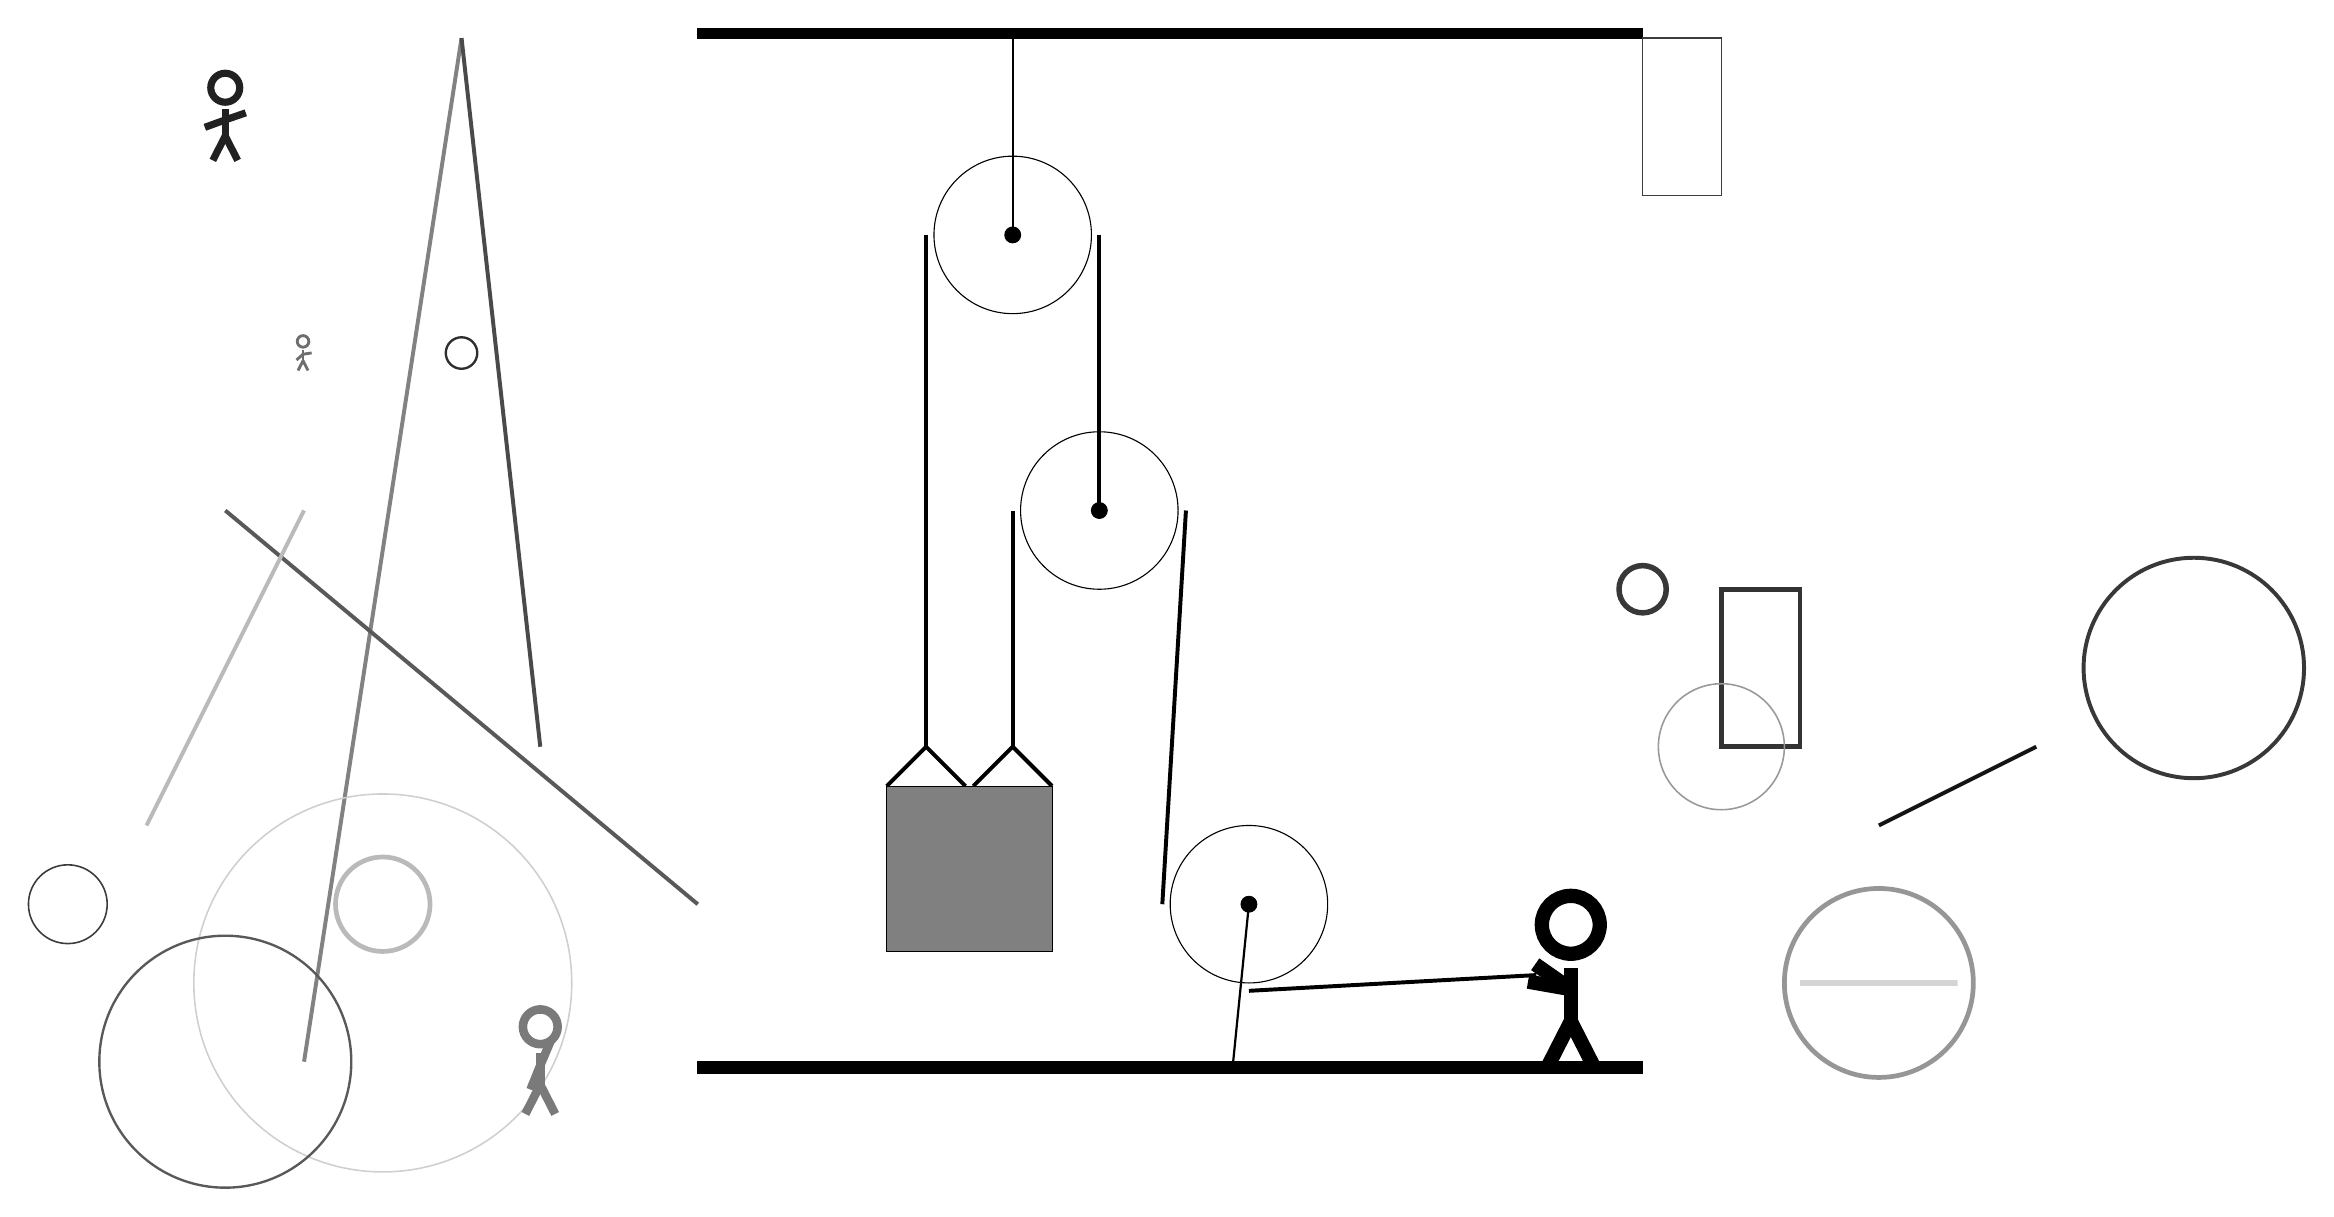
\begin{tikzpicture}
			%%%%% START %%%%%
			
			\draw[fill=black] (-2, 10) rectangle (10, 10.125);
			
			\draw (2, 7.5) circle (1);
			\draw[fill=black] (2, 7.5) circle (0.1);
			\draw[thick] (2, 7.5) -- (2, 10);
			
			\draw (3.1, 4.0) circle (1);
			\draw[fill=black] (3.1, 4.0) circle (0.1);
			
			\draw (5, -1) circle (1);
			\draw[fill=black] (5, -1) circle (0.1);
			\draw[thick] (5, -1) -- (4.8, -3);
			
			\draw[line width = 0.5mm]  (0.4, 0.5) -- (0.9, 1.0) -- (1.4, 0.5);
			\draw[line width = 0.5mm]  (1.5, 0.5) -- (2.0, 1.0) -- (2.5, 0.5);
			\draw[fill=black!50] (0.4, 0.5) rectangle (2.5, -1.6);
			
			\draw[line width=0.5mm, color=black!49](-5, 10) -- (-7, -3);
			
			\node[line width=0.3mm, color=black!87] at (-8, 9) {\Strichmaxerl[5][20][19]};
			\draw[line width=0.7mm, color=black!17] (12, -2) rectangle (14, -2);
			\draw[line width=0.5mm, color=black!65](-2, -1) -- (-8, 4);
			\draw [line width=0.6mm, color=black!41](13, -2) circle (1.2);
			\draw [line width=0.2mm, color=black!19](-6, -2) circle (2.4);
			\draw[line width=0.2mm, color=black!76] (10, 10) rectangle (11, 8);
			
			\draw [line width=0.3mm, color=black!82](-5, 6) circle (0.2);
			\node[line width=0.5mm, color=black!52] at (-4, -3) {\Strichmaxerl[6][68][67]};
			
			\draw[line width=0.5mm, color=black!71](-5, 10) -- (-4, 1);
			\draw[line width=0.6mm, color=black!80] (12, 3) rectangle (11, 1);
			\draw[line width=0.5mm, color=black!27](-7, 4) -- (-9, 0);
			\draw [line width=0.7mm, color=black!78](10, 3) circle (0.3);
			\draw [line width=0.6mm, color=black!27](-6, -1) circle (0.6);
			\draw [line width=0.3mm, color=black!65](-8, -3) circle (1.6);
			\draw [line width=0.5mm, color=black!78](17, 2) circle (1.4);
			
			\node[line width=0.3mm, color=black!57] at (-7, 6) {\Strichmaxerl[2][41][9]};
			\draw [line width=0.2mm, color=black!40](11, 1) circle (0.8);
			\draw[line width=0.5mm, color=black!92](13, 0) -- (15, 1);
			
			\draw [line width=0.2mm, color=black!77](-10, -1) circle (0.5);
			
			\draw[line width = 0.5mm] (0.9, 7.5) -- (0.9, 1.0);
			\centerarc[line width = 0.5mm](2, 7.5)(0:180:1.1);
			\draw[line width = 0.5mm] (3.1, 7.5) -- (3.1, 4.0);
			\draw[line width = 0.5mm] (2.0, 4.0) -- (2.0, 1.0);
			\centerarc[line width = 0.5mm](3.1, 4.0)(0:180:1.1);
			\draw[line width = 0.5mm] (4.2, 4.0) -- (3.9, -1);
			\centerarc[line width = 0.5mm](5, -1)(180:270:1.1);
			\draw[line width = 0.5mm] (5, -2.1) -- (8.65, -1.9);
			
			\node at (9, -2) {\Strichmaxerl[10][-35][170]};
			
			\draw[fill=black] (-2, -3) rectangle (10, -3.15);
			
			%%%%% END %%%%%
		\end{tikzpicture}
	\end{figure}	
\end{document}